\documentclass[11pt]{article}
\usepackage[utf8]{inputenc}
\usepackage[margin=1in]{geometry}
\usepackage{graphicx}
\usepackage{titlesec}
\usepackage{hyperref}
\usepackage{booktabs}
\usepackage{caption}
\usepackage{float}
\usepackage{amsmath}

% Title Configuration
\title{CS 5330: Computer Vision \\ \textbf{Project 5: Recognition using Deep Networks}}
\author{Varun Reddy Patlolla \and Anand Pinnamaneni}
\date{April 7, 2026}

\begin{document}

\maketitle

\section{Project Description}

This project explores building, training, analyzing, and modifying deep networks for digit recognition using the MNIST dataset. The MNIST dataset consists of 60,000 training images and 10,000 test images of handwritten digits (0--9), each 28$\times$28 pixels in grayscale. We implement a Convolutional Neural Network (CNN) for digit classification, evaluate its performance, test on custom handwritten digits, and re-implement the recognition task using a Vision Transformer (ViT) architecture.

All code is written in Python using PyTorch and torchvision, following a well-structured format with classes, functions, and a main entry point.

\section{Task 1: Build and Train a Network to Recognize Digits}

\subsection{Task 1A: Get the MNIST Digit Data Set}

The MNIST dataset was loaded directly from \texttt{torchvision.datasets.MNIST}. Images are normalized using a mean of 0.5 and standard deviation of 0.5. The first six example digits from the test set are visualized below using matplotlib's subplot functionality.

\begin{figure}[H]
    \centering
    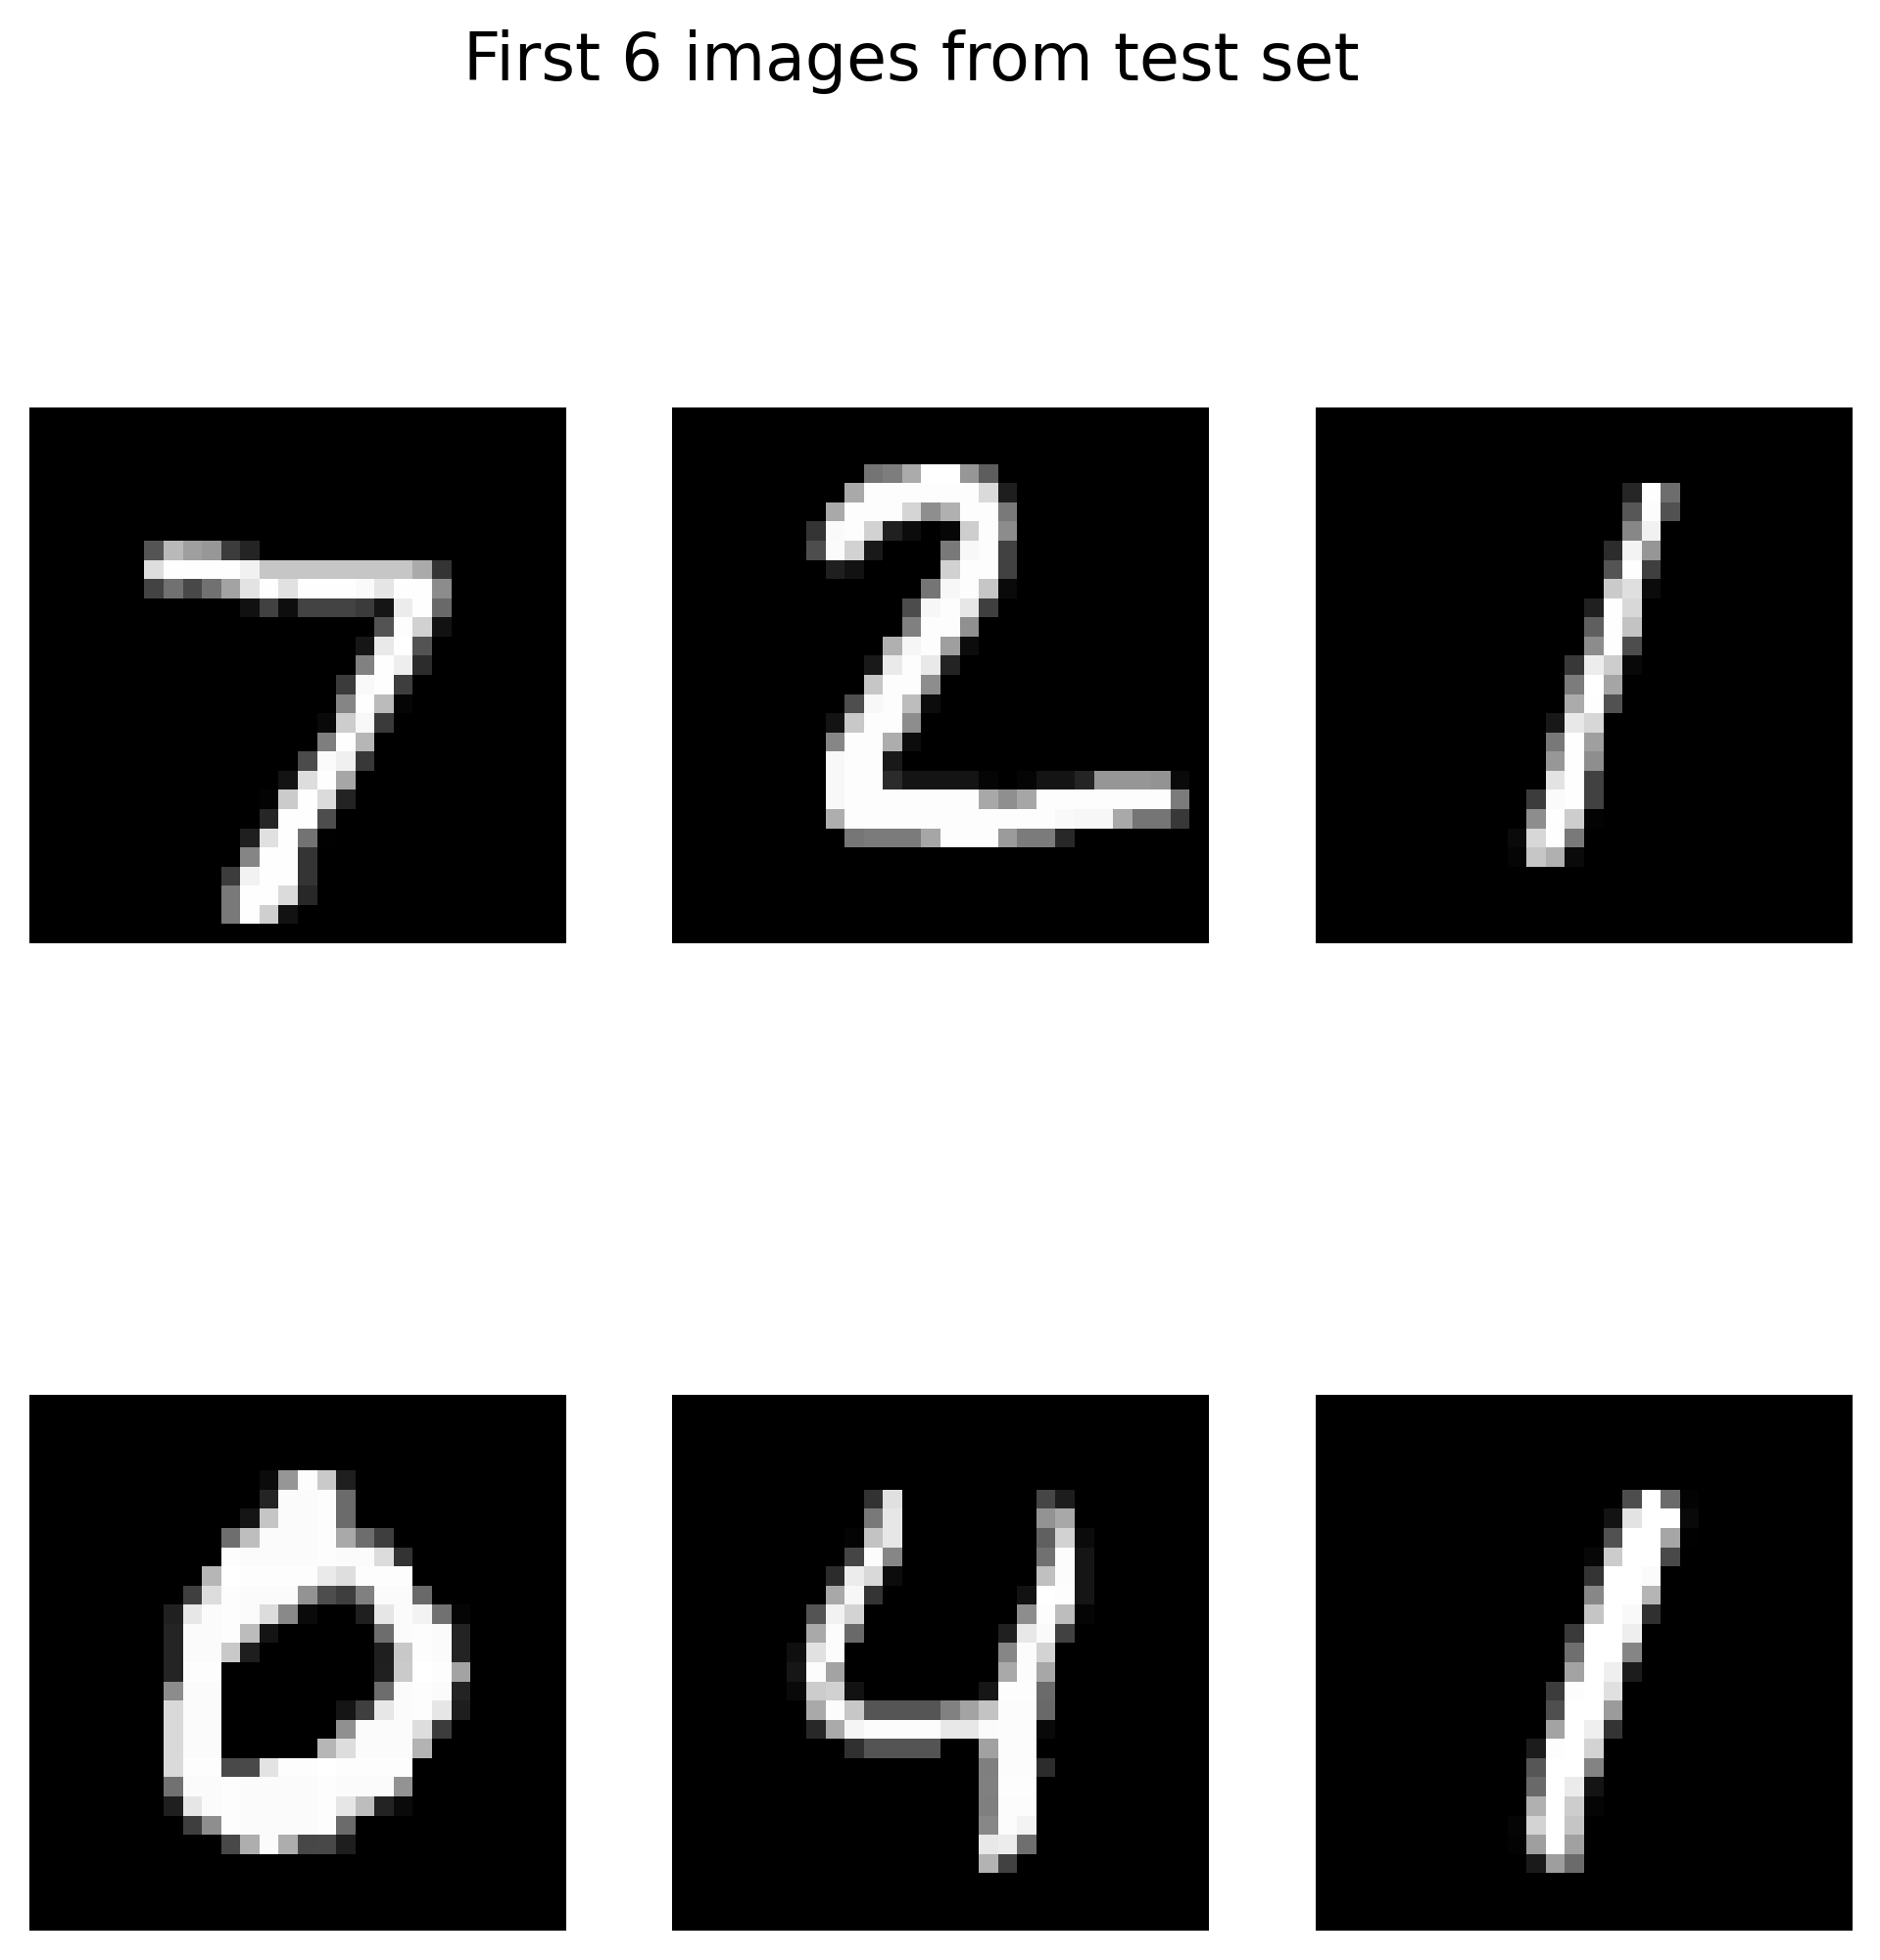
\includegraphics[width=0.65\textwidth]{results/task1A.png}
    \caption{First six example digits from the MNIST test set.}
\end{figure}

\subsection{Task 1B: Build a CNN Network Model}

We built a CNN model (\texttt{Net}) derived from \texttt{nn.Module} with the following architecture:

\begin{table}[H]
    \centering
    \caption{CNN Network Architecture}
    \vspace{0.1in}
    \begin{tabular}{clc}
        \toprule
        \textbf{Layer} & \textbf{Description} & \textbf{Output Shape} \\
        \midrule
        1 & Conv2d(1, 10, kernel\_size=5) & 10 $\times$ 24 $\times$ 24 \\
        2 & MaxPool2d(2) + ReLU & 10 $\times$ 12 $\times$ 12 \\
        3 & Conv2d(10, 20, kernel\_size=5) & 20 $\times$ 8 $\times$ 8 \\
        4 & Dropout2d(0.5) & 20 $\times$ 8 $\times$ 8 \\
        5 & MaxPool2d(2) + ReLU & 20 $\times$ 4 $\times$ 4 \\
        6 & Flatten + Linear(320, 50) + ReLU & 50 \\
        7 & Linear(50, 10) + LogSoftmax & 10 \\
        \bottomrule
    \end{tabular}
\end{table}

The first convolution layer applies 10 filters of size 5$\times$5 to extract low-level features such as edges and corners. The second convolution layer applies 20 filters of size 5$\times$5 to capture higher-level patterns. Max pooling reduces spatial dimensions by half at each stage, and the dropout layer (50\% rate) helps prevent overfitting during training. The final fully connected layers map the 320-dimensional flattened feature vector to 10 output classes via a 50-node hidden layer.

\begin{figure}[H]
    \centering
    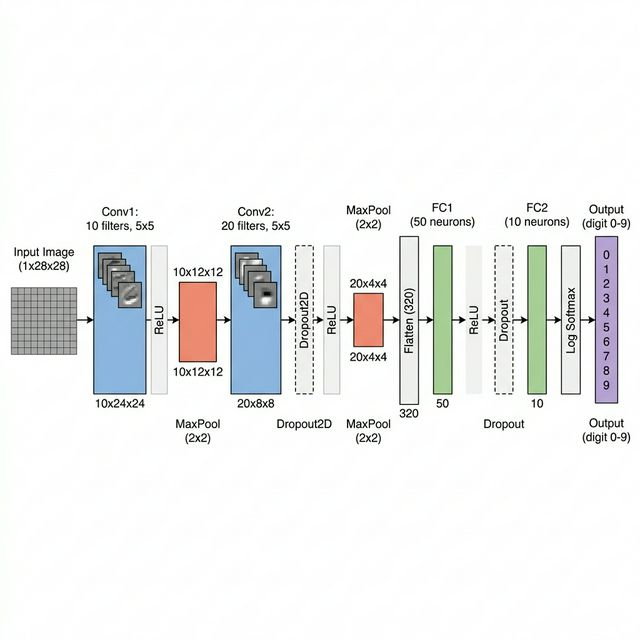
\includegraphics[width=0.85\textwidth]{results/cnn_architecture.png}
    \caption{CNN network architecture diagram. Input flows from left to right through two convolution-pooling stages, followed by fully connected classification layers.}
\end{figure}

\subsection{Task 1C: Train the Model}

The model was trained for 5 epochs with the following hyperparameters:

\begin{table}[H]
    \centering
    \caption{CNN Training Hyperparameters}
    \vspace{0.1in}
    \begin{tabular}{lc}
        \toprule
        \textbf{Parameter} & \textbf{Value} \\
        \midrule
        Optimizer & SGD \\
        Learning Rate & 0.01 \\
        Batch Size & 64 \\
        Loss Function & Negative Log Likelihood (NLLLoss) \\
        Epochs & 5 \\
        \bottomrule
    \end{tabular}
\end{table}

The training and test loss were recorded after each epoch. The plot below shows the training loss (blue line, sampled every 100 batches) and test loss (red dots, evaluated after each epoch).

\begin{figure}[H]
    \centering
    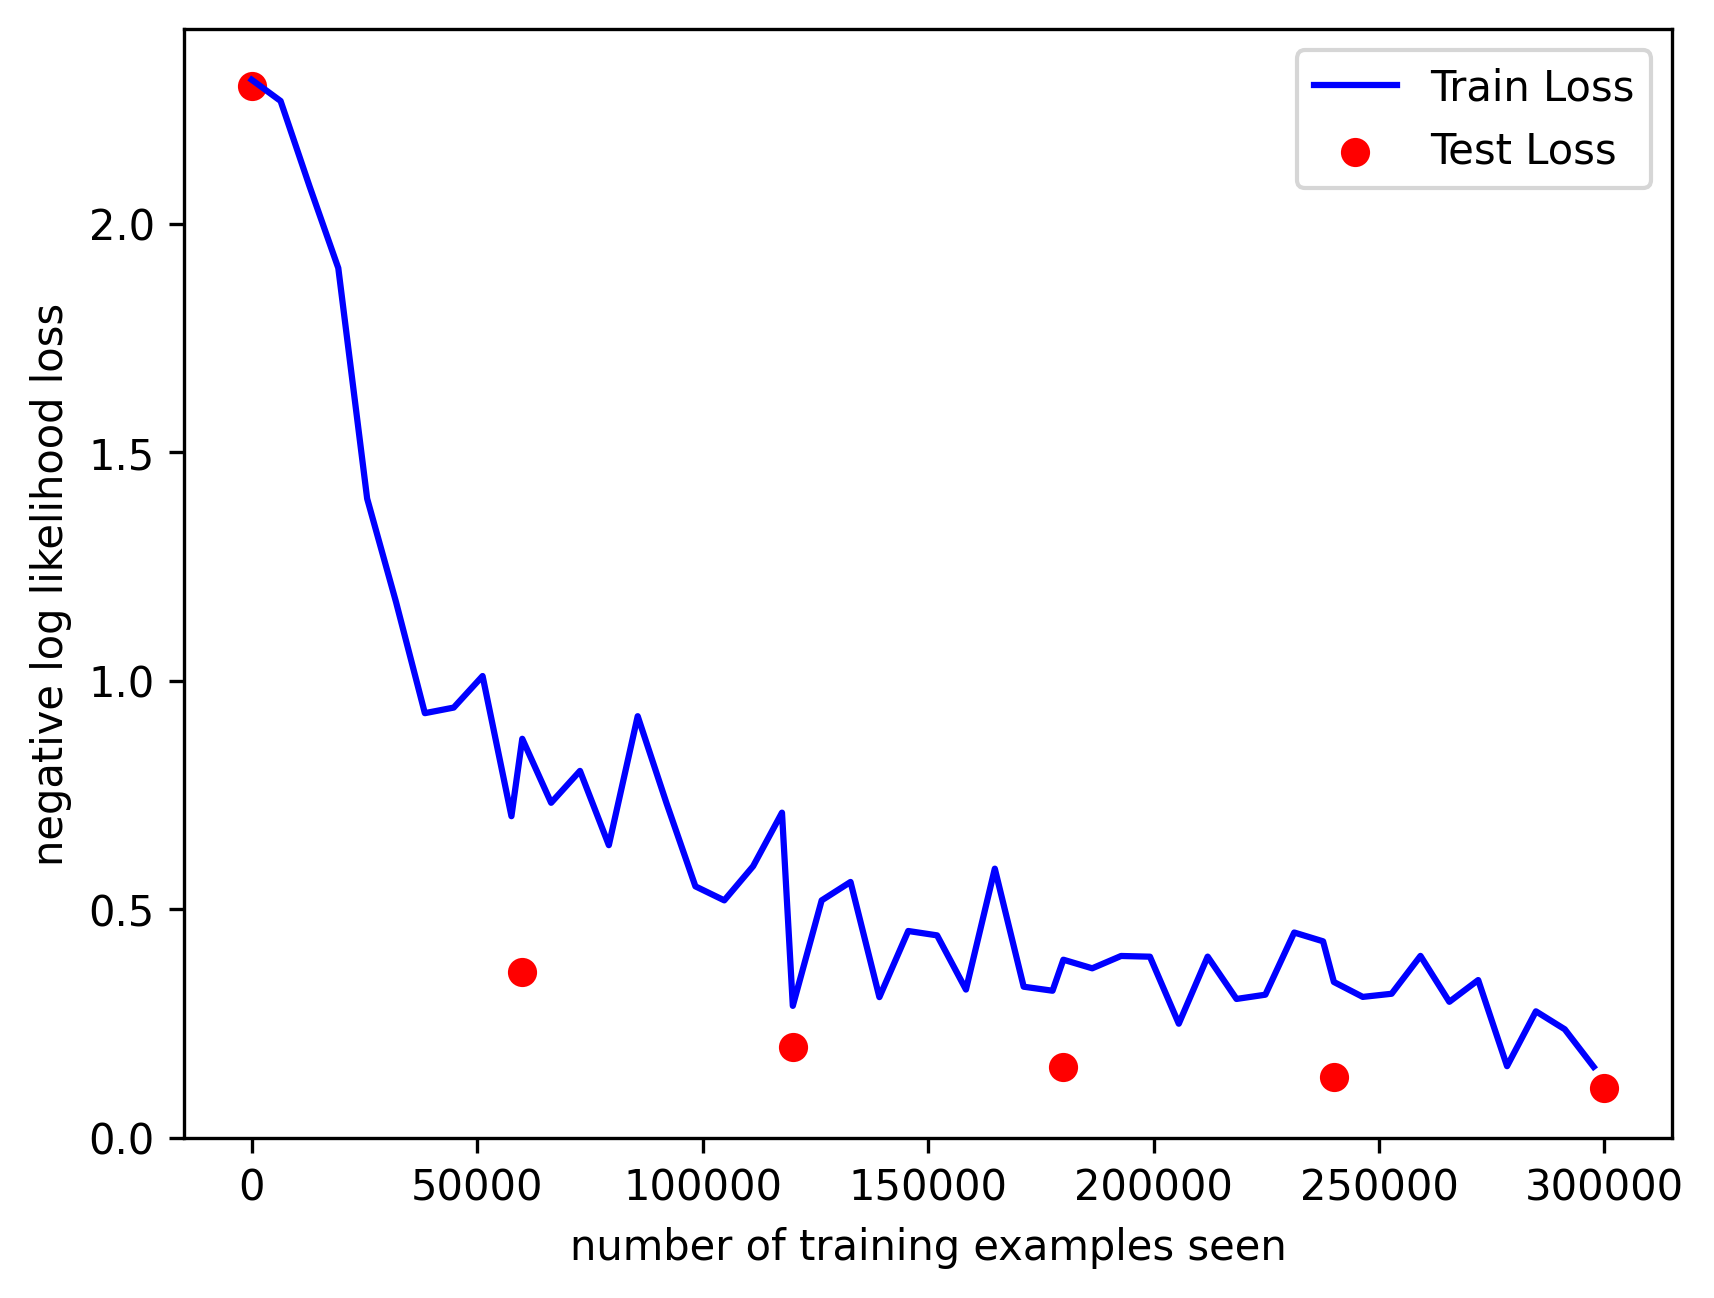
\includegraphics[width=0.75\textwidth]{results/training_performance.png}
    \caption{CNN training and test loss over 5 epochs. The training loss decreases rapidly in the first epoch and continues to decline. Test loss consistently decreases, indicating good generalization.}
\end{figure}

The training loss starts at approximately 2.3 (random initialization) and drops to below 0.5 after the first epoch. By epoch 5, the training loss fluctuates around 0.2--0.5, and the test loss stabilizes near 0.1, indicating the network has learned to classify digits effectively without overfitting. The final test accuracy of the CNN was approximately \textbf{96.40\%}. % TODO: Replace with actual CNN accuracy

\subsection{Task 1D: Save the Network}

After training, the model's learned parameters (\texttt{state\_dict}) were saved to \texttt{mnist\_model\_weights.pth} using \texttt{torch.save()}. This allows the network to be reloaded later without retraining.

\subsection{Task 1E: Read the Network and Run on Test Set}

In a separate file (\texttt{task1.E.py}), the saved network was loaded and set to evaluation mode using \texttt{model.eval()}. This is critical because evaluation mode disables dropout---instead of randomly zeroing values, it multiplies each value by $(1 - \text{dropout rate})$ to produce deterministic outputs.

The network was run on the first 10 test examples. For each image, the program prints the 10 network output values (log probabilities, 2 decimal places), the predicted digit (index of maximum output), and the correct label.

\begin{figure}[H]
    \centering
    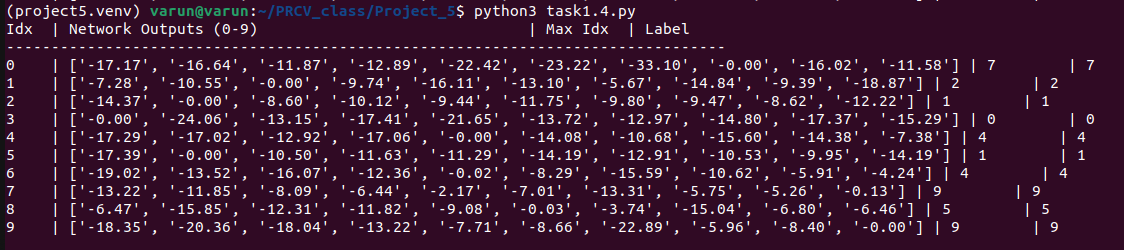
\includegraphics[width=0.95\textwidth]{results/task1.4_table.png}
    \caption{Terminal output showing the 10 log-softmax values, predicted digit, and correct label for the first 10 test examples. The network correctly classifies all 10 digits.}
\end{figure}

The first 9 test digits are also displayed in a 3$\times$3 grid with predictions:

\begin{figure}[H]
    \centering
    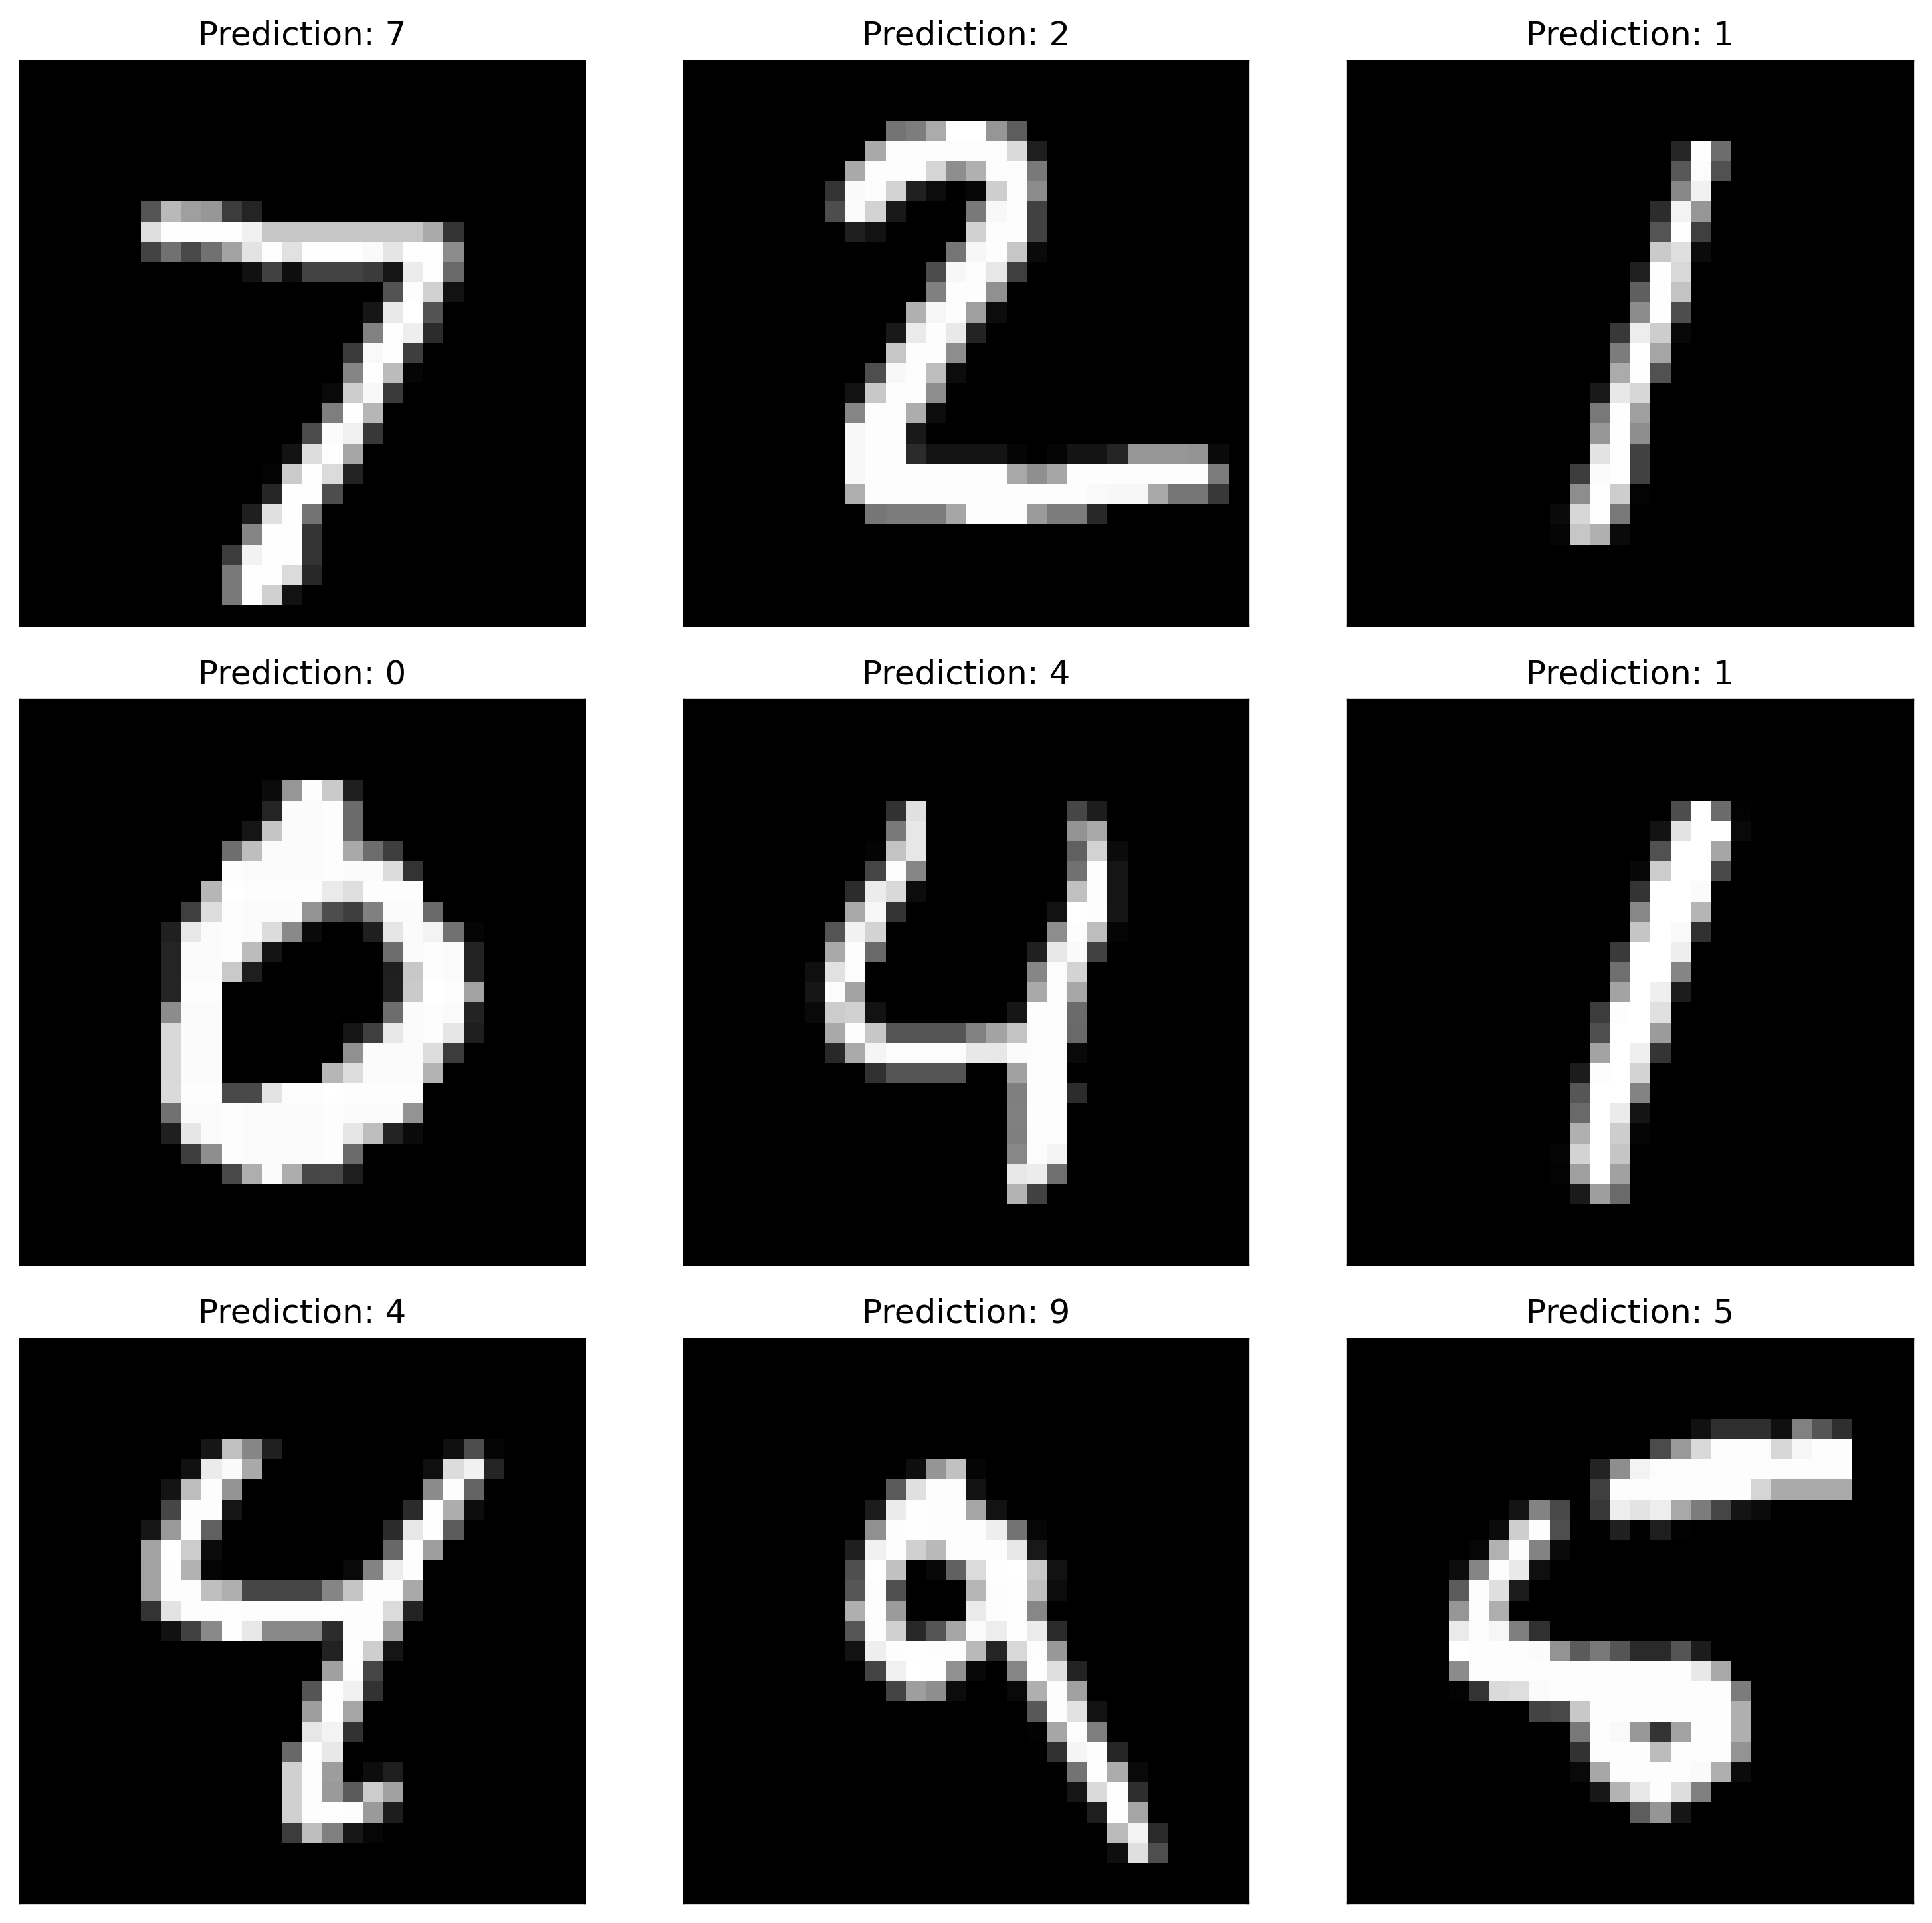
\includegraphics[width=0.65\textwidth]{results/test_predictions_grid.png}
    \caption{First 9 digits from the MNIST test set with network predictions. All predictions match the ground truth labels.}
\end{figure}

Looking at the output values, the network produces very confident predictions---the winning class typically has a log probability near 0.00 (probability close to 1.0), while all other classes have large negative values (probabilities close to 0). This demonstrates that the CNN has learned strong discriminative features for each digit class.

\subsection{Task 1F: Test the Network on New Inputs}

Ten handwritten digits (0--9) were written by hand on white paper using a thick marker, photographed, and cropped into individual square images. Each image was processed through the following pipeline:

\begin{enumerate}
    \item Convert to grayscale (single channel)
    \item Resize to 28$\times$28 pixels
    \item Normalize with mean=0.5 and std=0.5 to match MNIST intensity scaling
\end{enumerate}

Since the MNIST digits are white on a black background, the preprocessing ensures the handwritten images match this convention after transformation.

\begin{figure}[H]
    \centering
    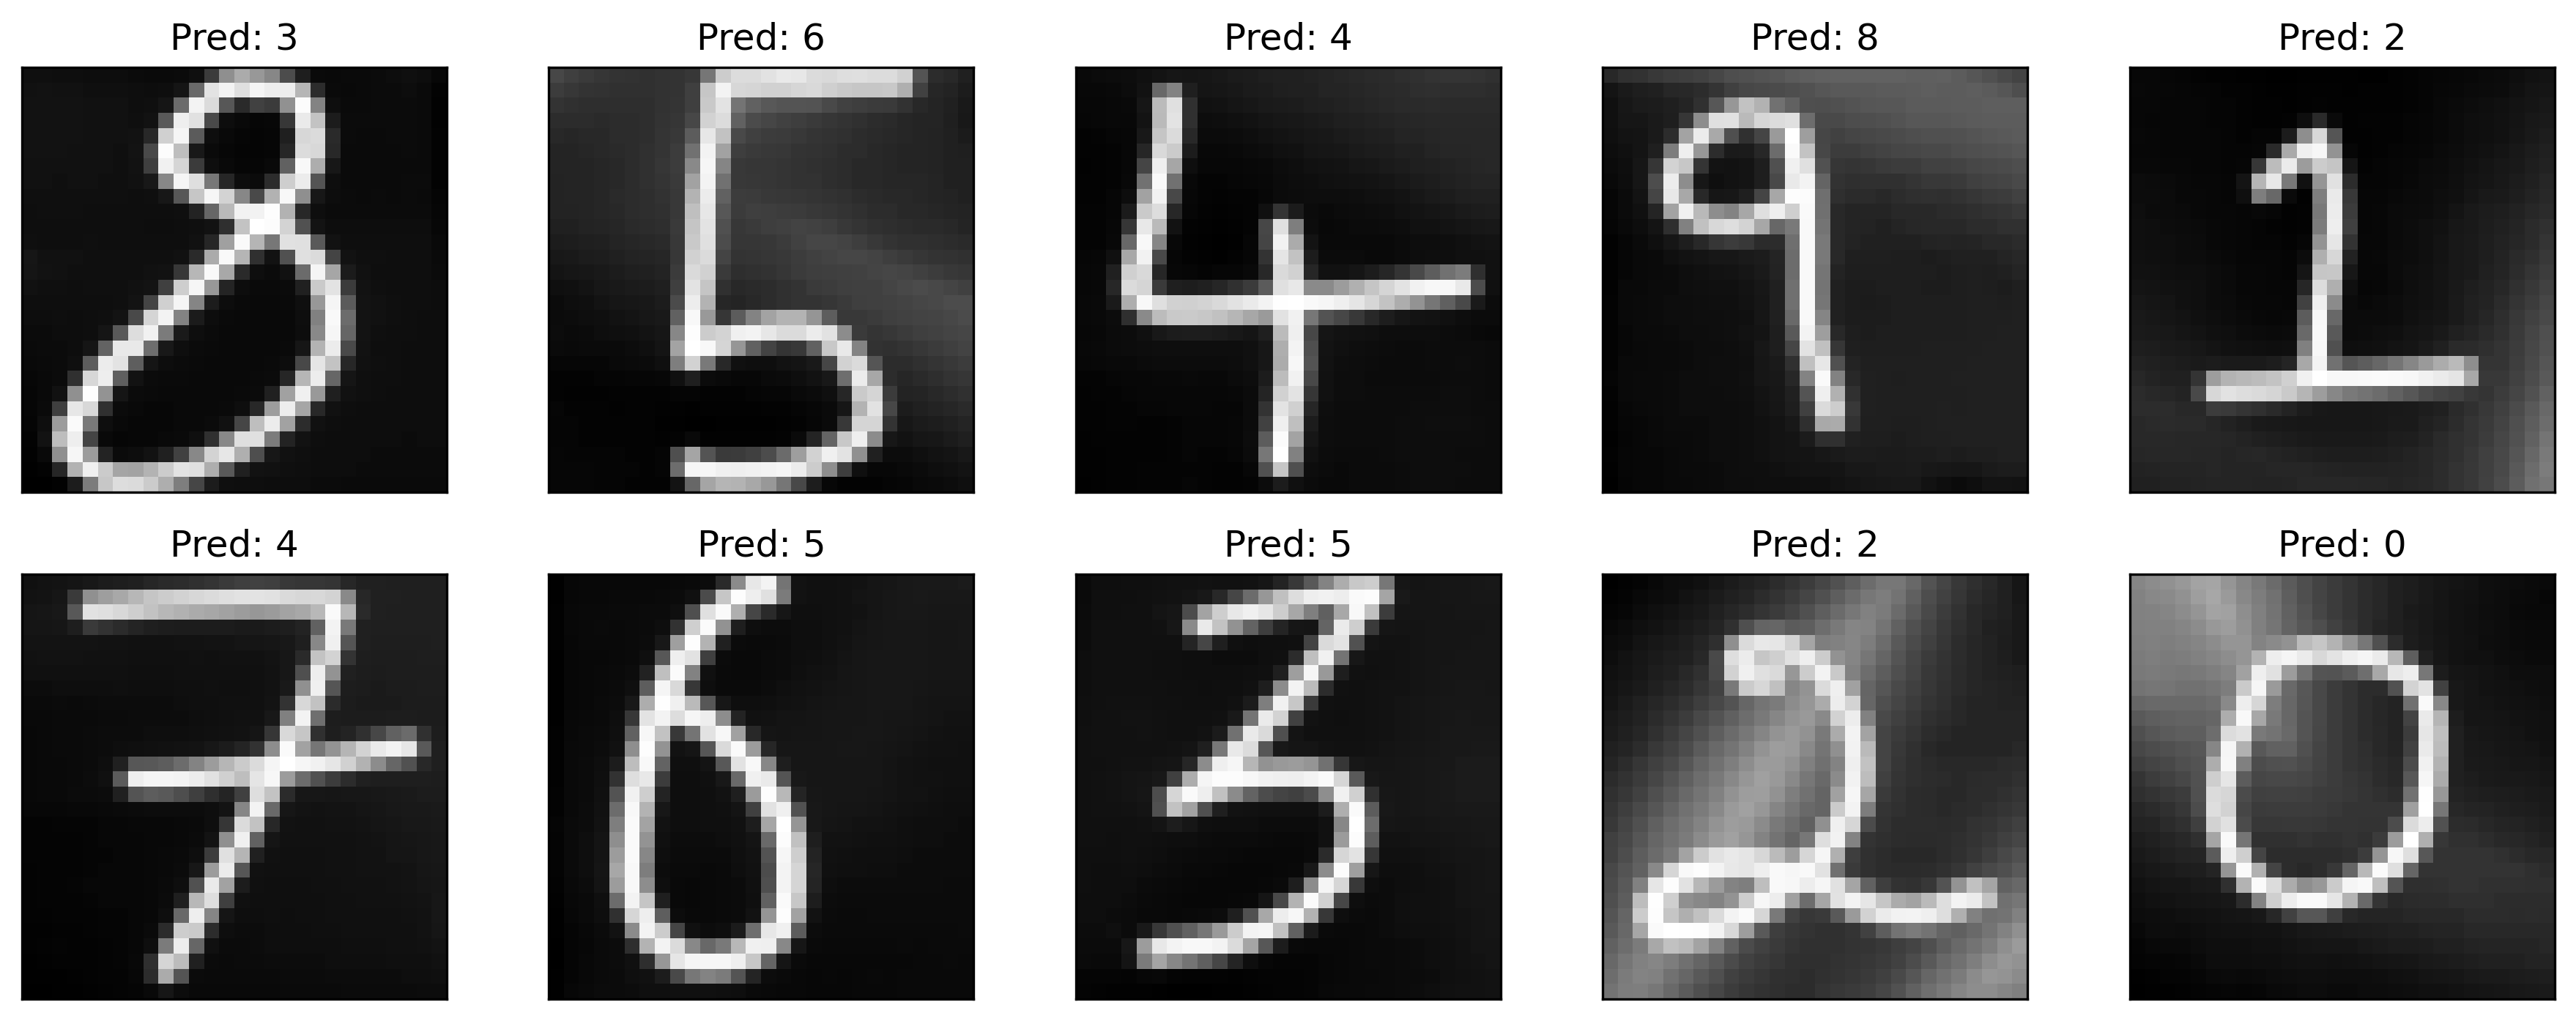
\includegraphics[width=0.95\textwidth]{results/custom_digit_test.png}
    \caption{Custom handwritten digits tested on the trained CNN. Predictions are shown above each image. Some digits are misclassified due to style differences from the MNIST training data.}
\end{figure}

\subsubsection{Analysis of Custom Digit Results}

The network struggles with several of the custom handwritten digits. Looking at the results:

\begin{itemize}
    \item Digits like \textbf{4}, \textbf{5}, \textbf{2}, and \textbf{0} are correctly recognized, as their shapes closely resemble typical MNIST examples.
    \item Digits like \textbf{8} (predicted as 3), \textbf{9} (predicted as 8), and \textbf{7} (predicted as 4) are misclassified. This is likely because:
    \begin{itemize}
        \item The handwriting style differs from the MNIST distribution (which is based on American census data from the 1990s)
        \item Stroke thickness and positioning vary from the training data
        \item The cropping and resizing may have introduced artifacts
    \end{itemize}
\end{itemize}

These results highlight the domain gap between the MNIST training data and real-world handwriting. The network has learned features specific to the MNIST style and does not generalize perfectly to all handwriting variations.

\section{Task 2: Examine Your Network}

% TODO: Add analysis of learned filters, feature maps, and truncated network outputs.

\subsection{Filter Visualization}

% TODO: Visualize the weights of the first convolutional layer filters.

\subsection{Effect of Filters on Test Images}

% TODO: Apply filters to a test image and show the resulting feature maps.

\subsection{Truncated Model Analysis}

% TODO: Build a truncated model (remove last classification layer), run test images through it,
% and analyze the resulting feature representations.

\section{Task 3: Transfer Learning on Greek Letters}

% TODO: Implement transfer learning from the MNIST CNN to classify Greek letters.

\subsection{Dataset Preparation}

% TODO: Describe how the Greek letter dataset was prepared and preprocessed.

\subsection{Network Modification}

% TODO: Describe how the pre-trained MNIST network was modified for Greek letter classification
% (freezing layers, replacing the last layer, etc.)

\subsection{Training and Results}

% TODO: Show training results and accuracy on Greek letter classification.

\section{Task 4: Re-implement the Network Using Transformer Layers}


\subsection{Transformer Architecture Overview}

For Task 4, we replaced the CNN with a Vision Transformer (ViT) that processes the image as a sequence of patch tokens rather than using convolution filters. The transformer architecture involves four key design steps:

\begin{enumerate}
    \item \textbf{Tokenization}: The 28$\times$28 image is divided into non-overlapping 7$\times$7 patches, producing 16 patches total. Each patch is flattened to a 49-dimensional vector and projected into a 64-dimensional embedding space via a linear layer.
    
    \item \textbf{Positional Embedding}: A learnable positional embedding is added to each token so the transformer knows the spatial location of each patch.
    
    \item \textbf{Transformer Encoder}: The tokens are processed through a stack of Transformer Encoder layers, each containing multi-head self-attention and a feedforward network with residual connections and layer normalization.
    
    \item \textbf{Classification}: The output tokens are averaged (mean pooling) into a single representation vector, which is passed through fully connected layers to produce the final 10-class prediction.
\end{enumerate}

\subsection{Default Settings}

The transformer was run with the following default configuration:

\begin{table}[H]
    \centering
    \caption{Transformer Network Configuration (Default Settings)}
    \vspace{0.1in}
    \begin{tabular}{lc}
        \toprule
        \textbf{Parameter} & \textbf{Value} \\
        \midrule
        Patch Size & 7 $\times$ 7 \\
        Number of Patches & 16 (4 $\times$ 4) \\
        Embedding Dimension & 64 \\
        Number of Attention Heads & 4 \\
        Number of Transformer Layers & 2 \\
        Feedforward Dimension & 256 (embed\_dim $\times$ 4) \\
        Dropout Rate & 0.1 (encoder), 0.5 (classifier) \\
        Pooling Strategy & Mean pooling (average all tokens) \\
        Classification Head & Linear(64, 50) $\rightarrow$ ReLU $\rightarrow$ Dropout $\rightarrow$ Linear(50, 10) \\
        \midrule
        Optimizer & Adam \\
        Learning Rate & 0.001 \\
        Batch Size & 64 \\
        Epochs & 10 \\
        Loss Function & NLLLoss \\
        \bottomrule
    \end{tabular}
\end{table}

\subsection{Model Architecture Printout}

\begin{verbatim}
NetTransformer(
  (patch_embedding): Linear(in_features=49, out_features=64)
  (transformer_encoder): TransformerEncoder(
    (layers): ModuleList(
      (0-1): 2 x TransformerEncoderLayer(
        (self_attn): MultiheadAttention(embed_dim=64, num_heads=4)
        (linear1): Linear(in_features=64, out_features=256)
        (linear2): Linear(in_features=256, out_features=64)
        (norm1): LayerNorm((64,))
        (norm2): LayerNorm((64,))
        (dropout): Dropout(p=0.1)
      )
    )
  )
  (fc1): Linear(in_features=64, out_features=50)
  (dropout): Dropout(p=0.5)
  (fc2): Linear(in_features=50, out_features=10)
)
\end{verbatim}

\subsection{Training Results}

\begin{figure}[H]
    \centering
    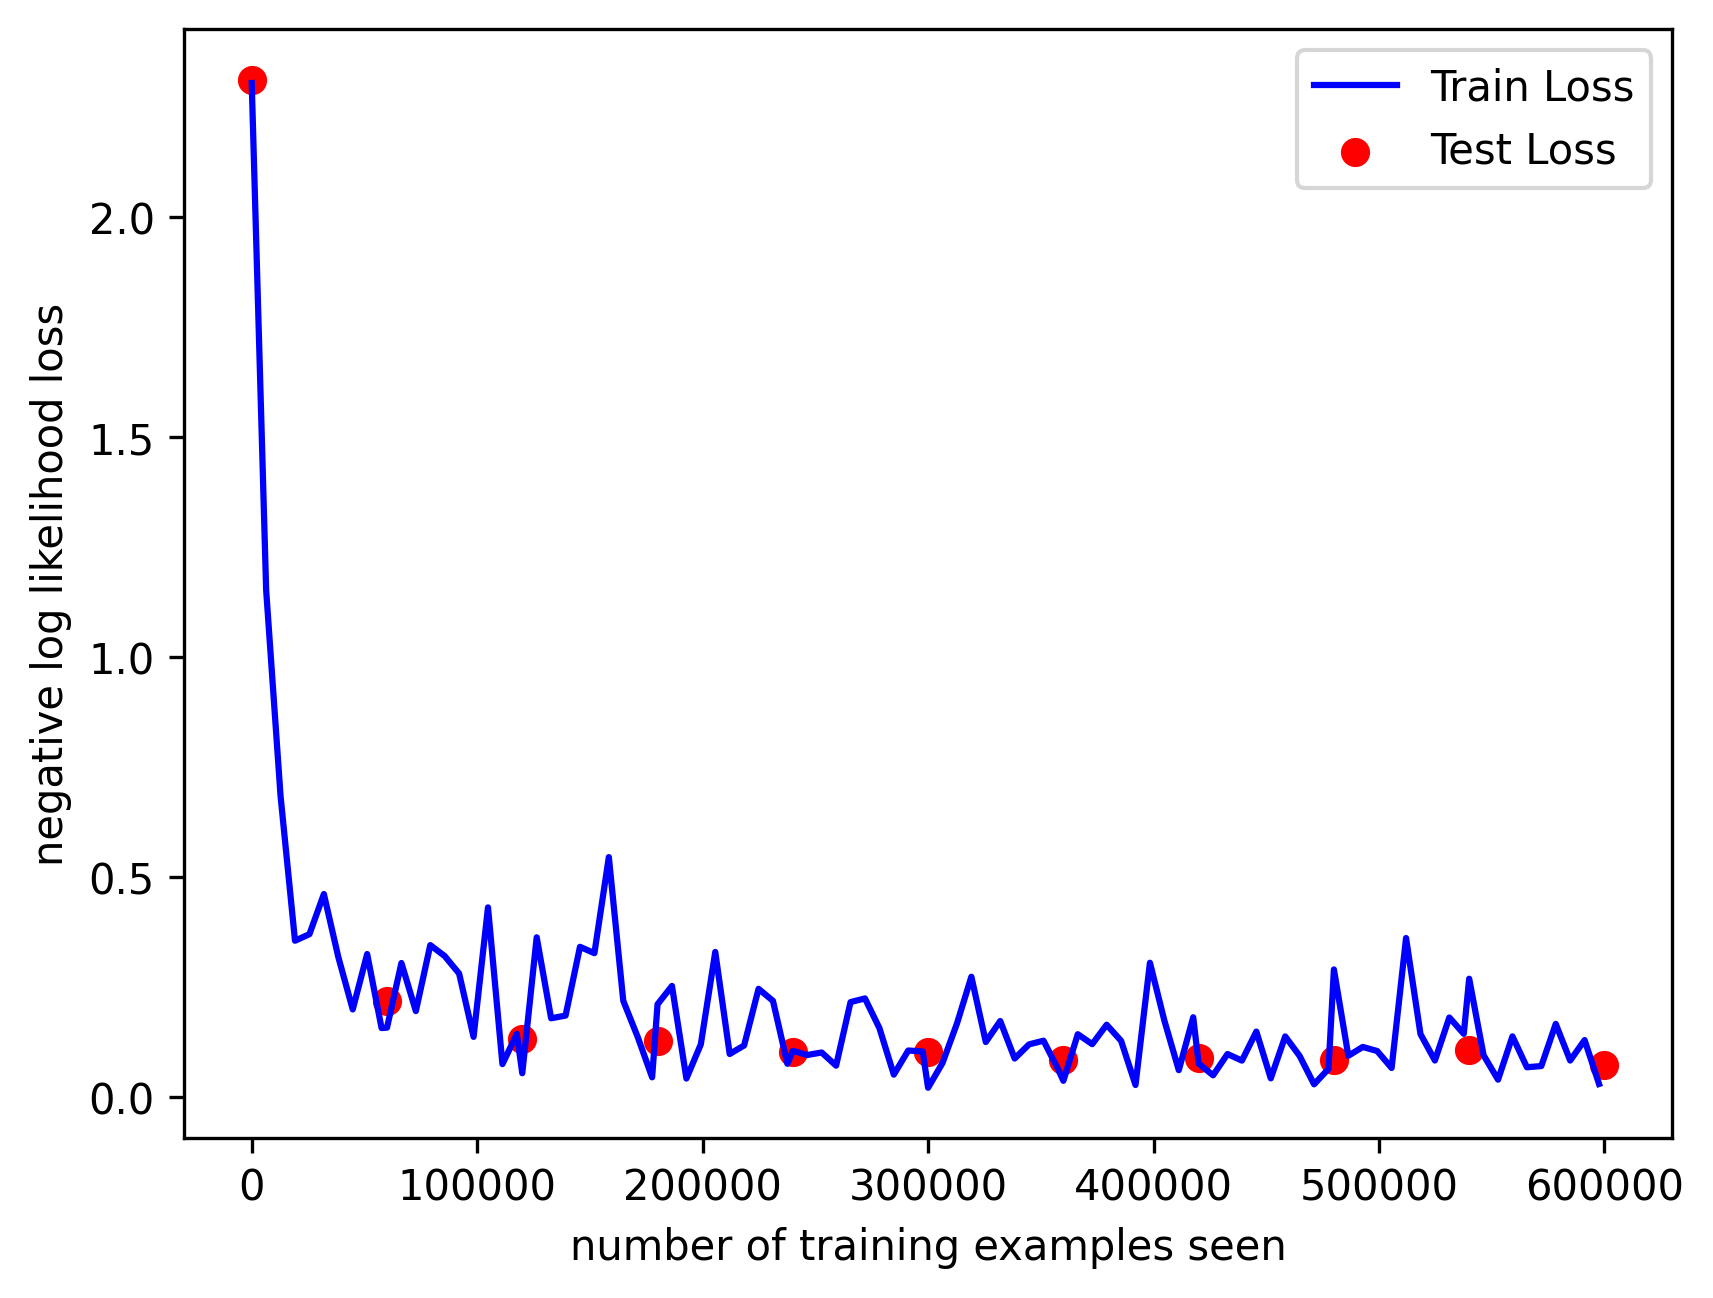
\includegraphics[width=0.75\textwidth]{results/training_performance_transformer.png}
    \caption{Transformer training and test loss over 10 epochs. The loss decreases rapidly in the first 1--2 epochs and stabilizes around 0.05--0.15. Final test accuracy: \textbf{97.92\%} (9792/10000).}
\end{figure}

The transformer training curve shows similar convergence behavior to the CNN, starting from a loss of approximately 2.3 and dropping rapidly. The model achieved a final test accuracy of \textbf{97.92\%} (9792/10000) with an average test loss of 0.0726. However, the training loss exhibits more oscillation (noise) compared to the CNN, which is typical for transformer architectures on small datasets like MNIST.

\subsection{Comparison: CNN vs.\ Transformer}

\begin{table}[H]
    \centering
    \caption{CNN vs.\ Transformer Comparison}
    \vspace{0.1in}
    \begin{tabular}{lcc}
        \toprule
        \textbf{Aspect} & \textbf{CNN} & \textbf{Transformer} \\
        \midrule
        Architecture & Convolutions + pooling & Self-attention + FFN \\
        Test Accuracy & 96.40\% & 97.92\% \\
        Parameters & $\sim$22K & $\sim$110K \\
        Training Epochs & 5 & 10 \\
        Optimizer & SGD (lr=0.01) & Adam (lr=0.001) \\
        Training Stability & Smooth convergence & Noisier convergence \\
        Inductive Bias & Local spatial features & Global attention patterns \\
        \bottomrule
    \end{tabular}
\end{table}

\subsubsection{Discussion}

The CNN and transformer achieve comparable accuracy on MNIST, but they approach the task differently:

\begin{itemize}
    \item \textbf{CNN}: Exploits local spatial structure through convolution filters that slide across the image. This inductive bias is well-suited for image tasks and allows the CNN to learn efficiently with fewer parameters and fewer training epochs.
    
    \item \textbf{Transformer}: Treats the image as a sequence of patches and uses self-attention to capture relationships between all patches simultaneously. This global receptive field is powerful but requires more parameters and training time to converge, especially on small datasets like MNIST.
    
    \item \textbf{Training dynamics}: The transformer's training curve is noisier because self-attention distributes learning across all patch pairs, making gradient updates less stable than the CNN's localized filter updates. Using the Adam optimizer (instead of SGD) helps mitigate this.
    
    \item \textbf{Scalability}: While both models perform well on MNIST, transformers typically excel on larger, more complex datasets (e.g., ImageNet) where global context matters more. For a simple 28$\times$28 digit recognition task, the CNN's local inductive bias is arguably more efficient.
\end{itemize}

\section{Task 5: Design Your Own Experiment}

% TODO: Describe your custom experiment comparing different architectures,
% hyperparameters, or training strategies.

\subsection{Experiment Design}

% TODO: State the hypothesis and experimental setup.

\subsection{Results and Analysis}

% TODO: Present and analyze the experiment results.

\section{Extensions}


\subsection{Extension A: Evaluating a Pre-trained Network's Convolutional Layers}

We loaded a pre-trained ResNet18 network from the PyTorch model zoo and visualized its first convolutional layer filters, comparing them to our MNIST CNN's learned filters.

ResNet18's first layer (\texttt{conv1}) is a Conv2d(3, 64, 7$\times$7) with stride 2 and padding 3---it has 64 filters operating on 3-channel RGB input, totaling 9,408 parameters. In contrast, our MNIST CNN's first layer is Conv2d(1, 10, 5$\times$5) with only 250 parameters.

\begin{figure}[H]
    \centering
    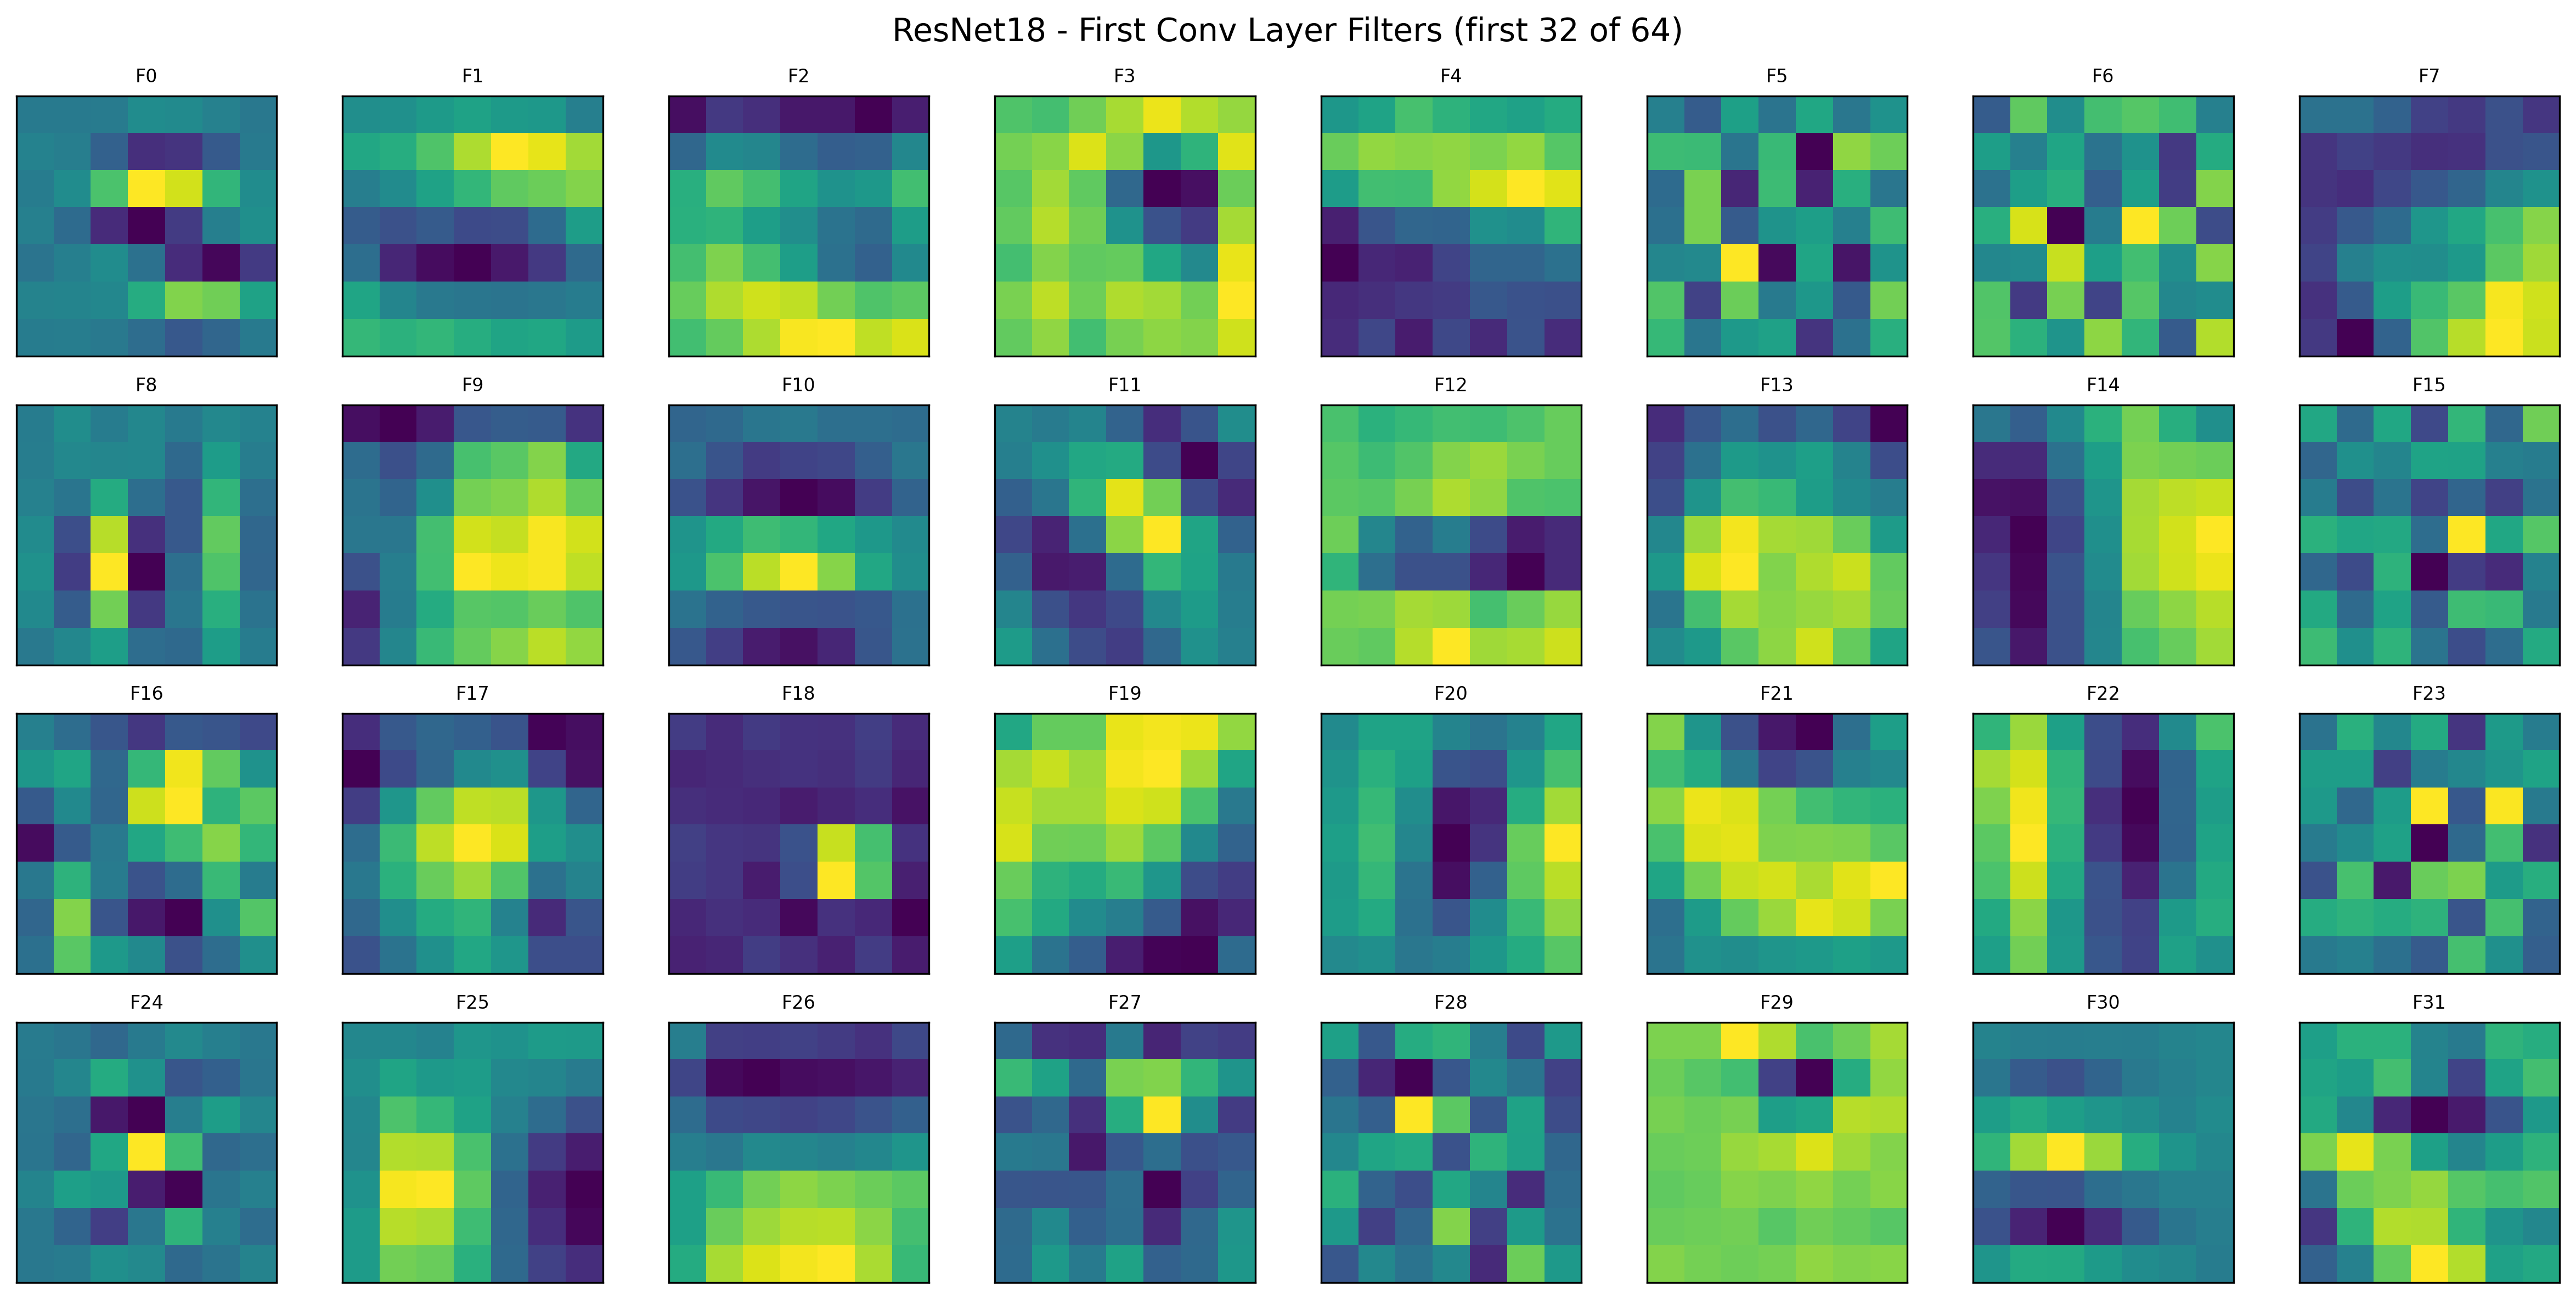
\includegraphics[width=0.95\textwidth]{results/resnet18_conv1_filters.png}
    \caption{First 32 of 64 filters from ResNet18's first convolutional layer (channel-averaged). Clear edge detectors, gradient filters, and blob detectors are visible, learned from ImageNet's 1.2M natural images.}
\end{figure}

\begin{figure}[H]
    \centering
    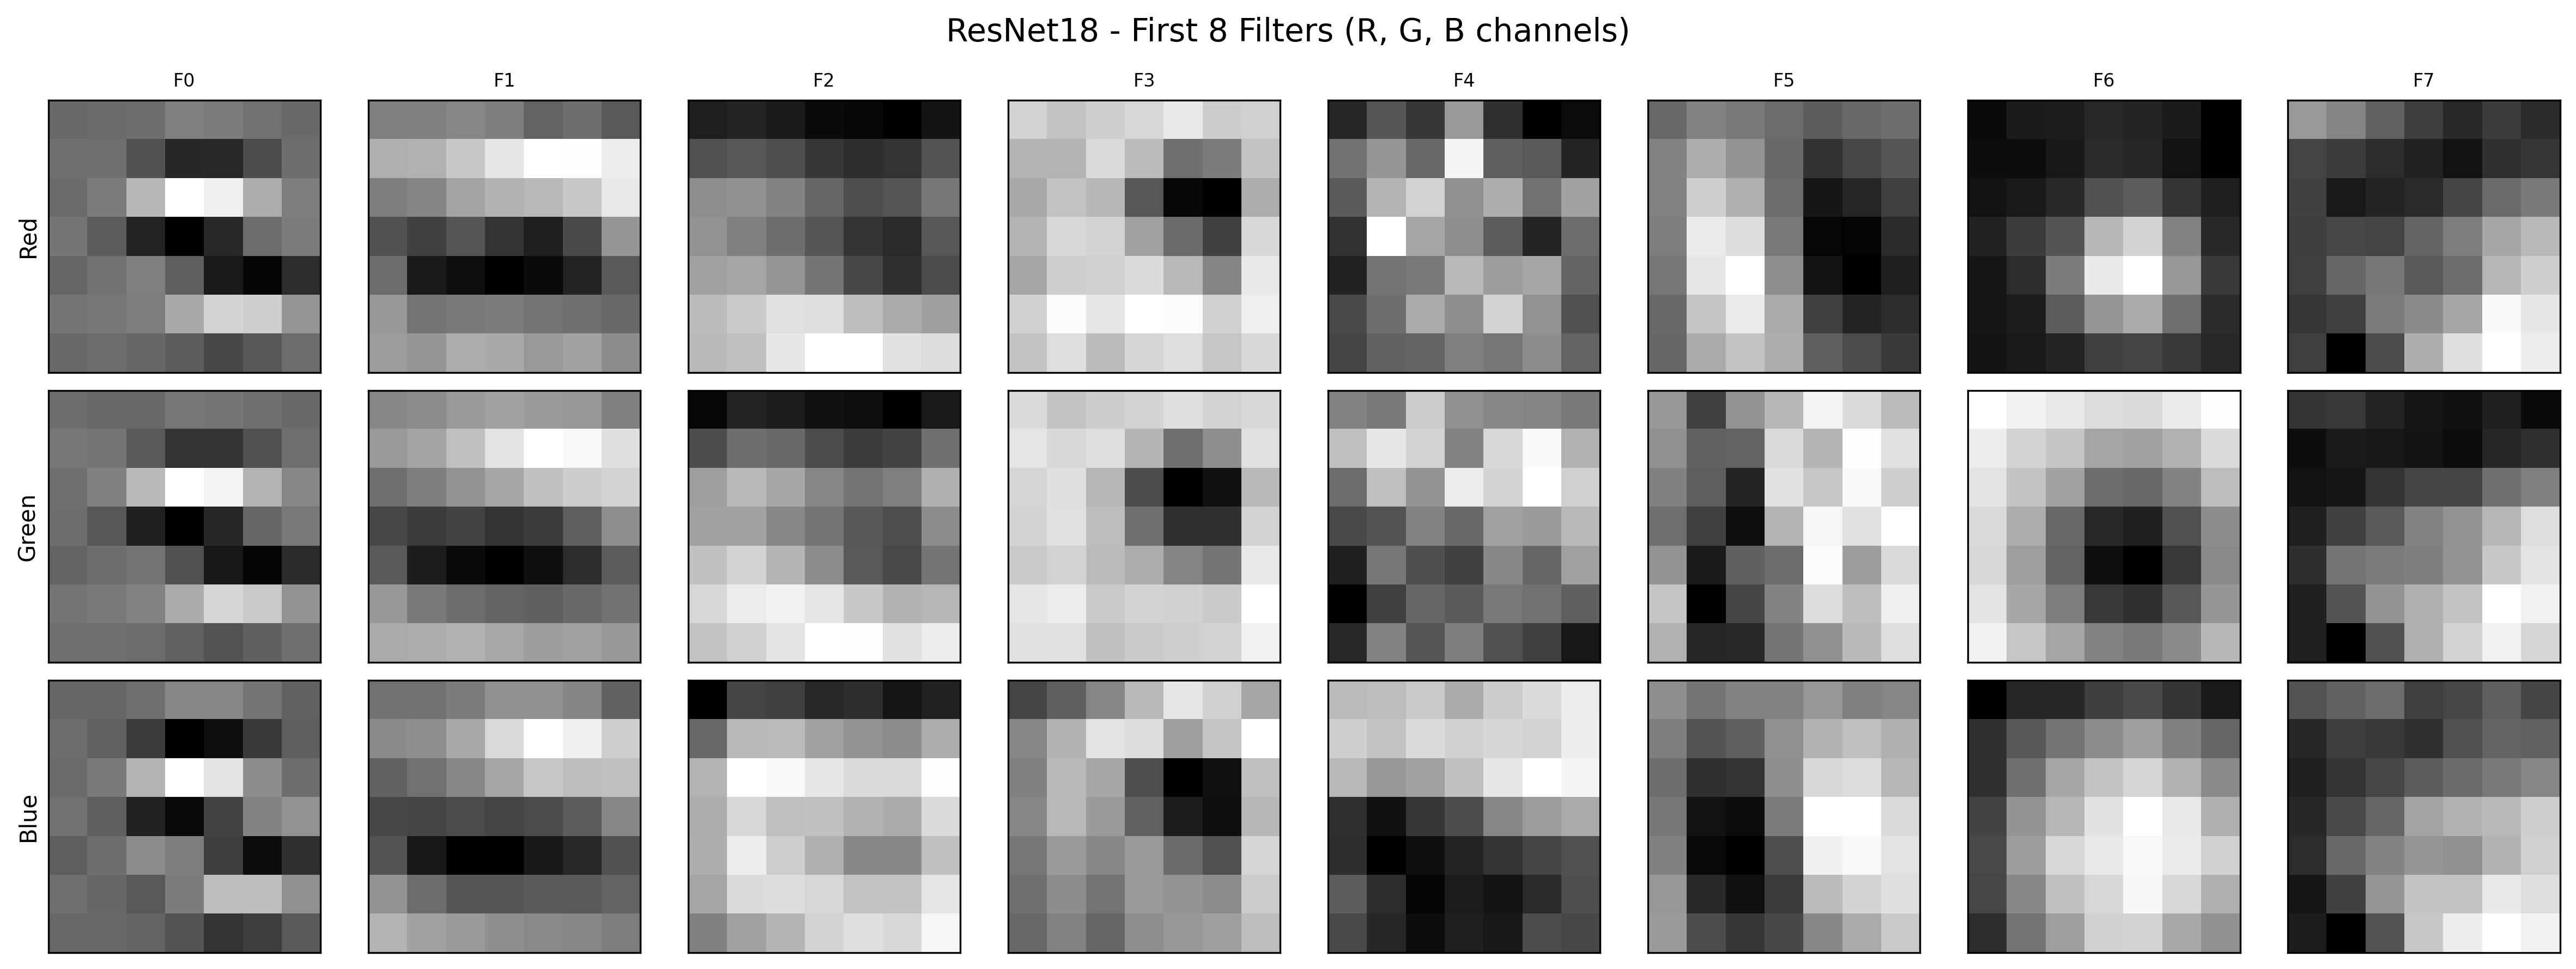
\includegraphics[width=0.95\textwidth]{results/resnet18_rgb_channels.png}
    \caption{First 8 ResNet18 filters separated by R, G, B channels. Different channels learn different color-specific features---some filters respond similarly across channels (luminance detectors) while others show color-opponent responses.}
\end{figure}

\begin{figure}[H]
    \centering
    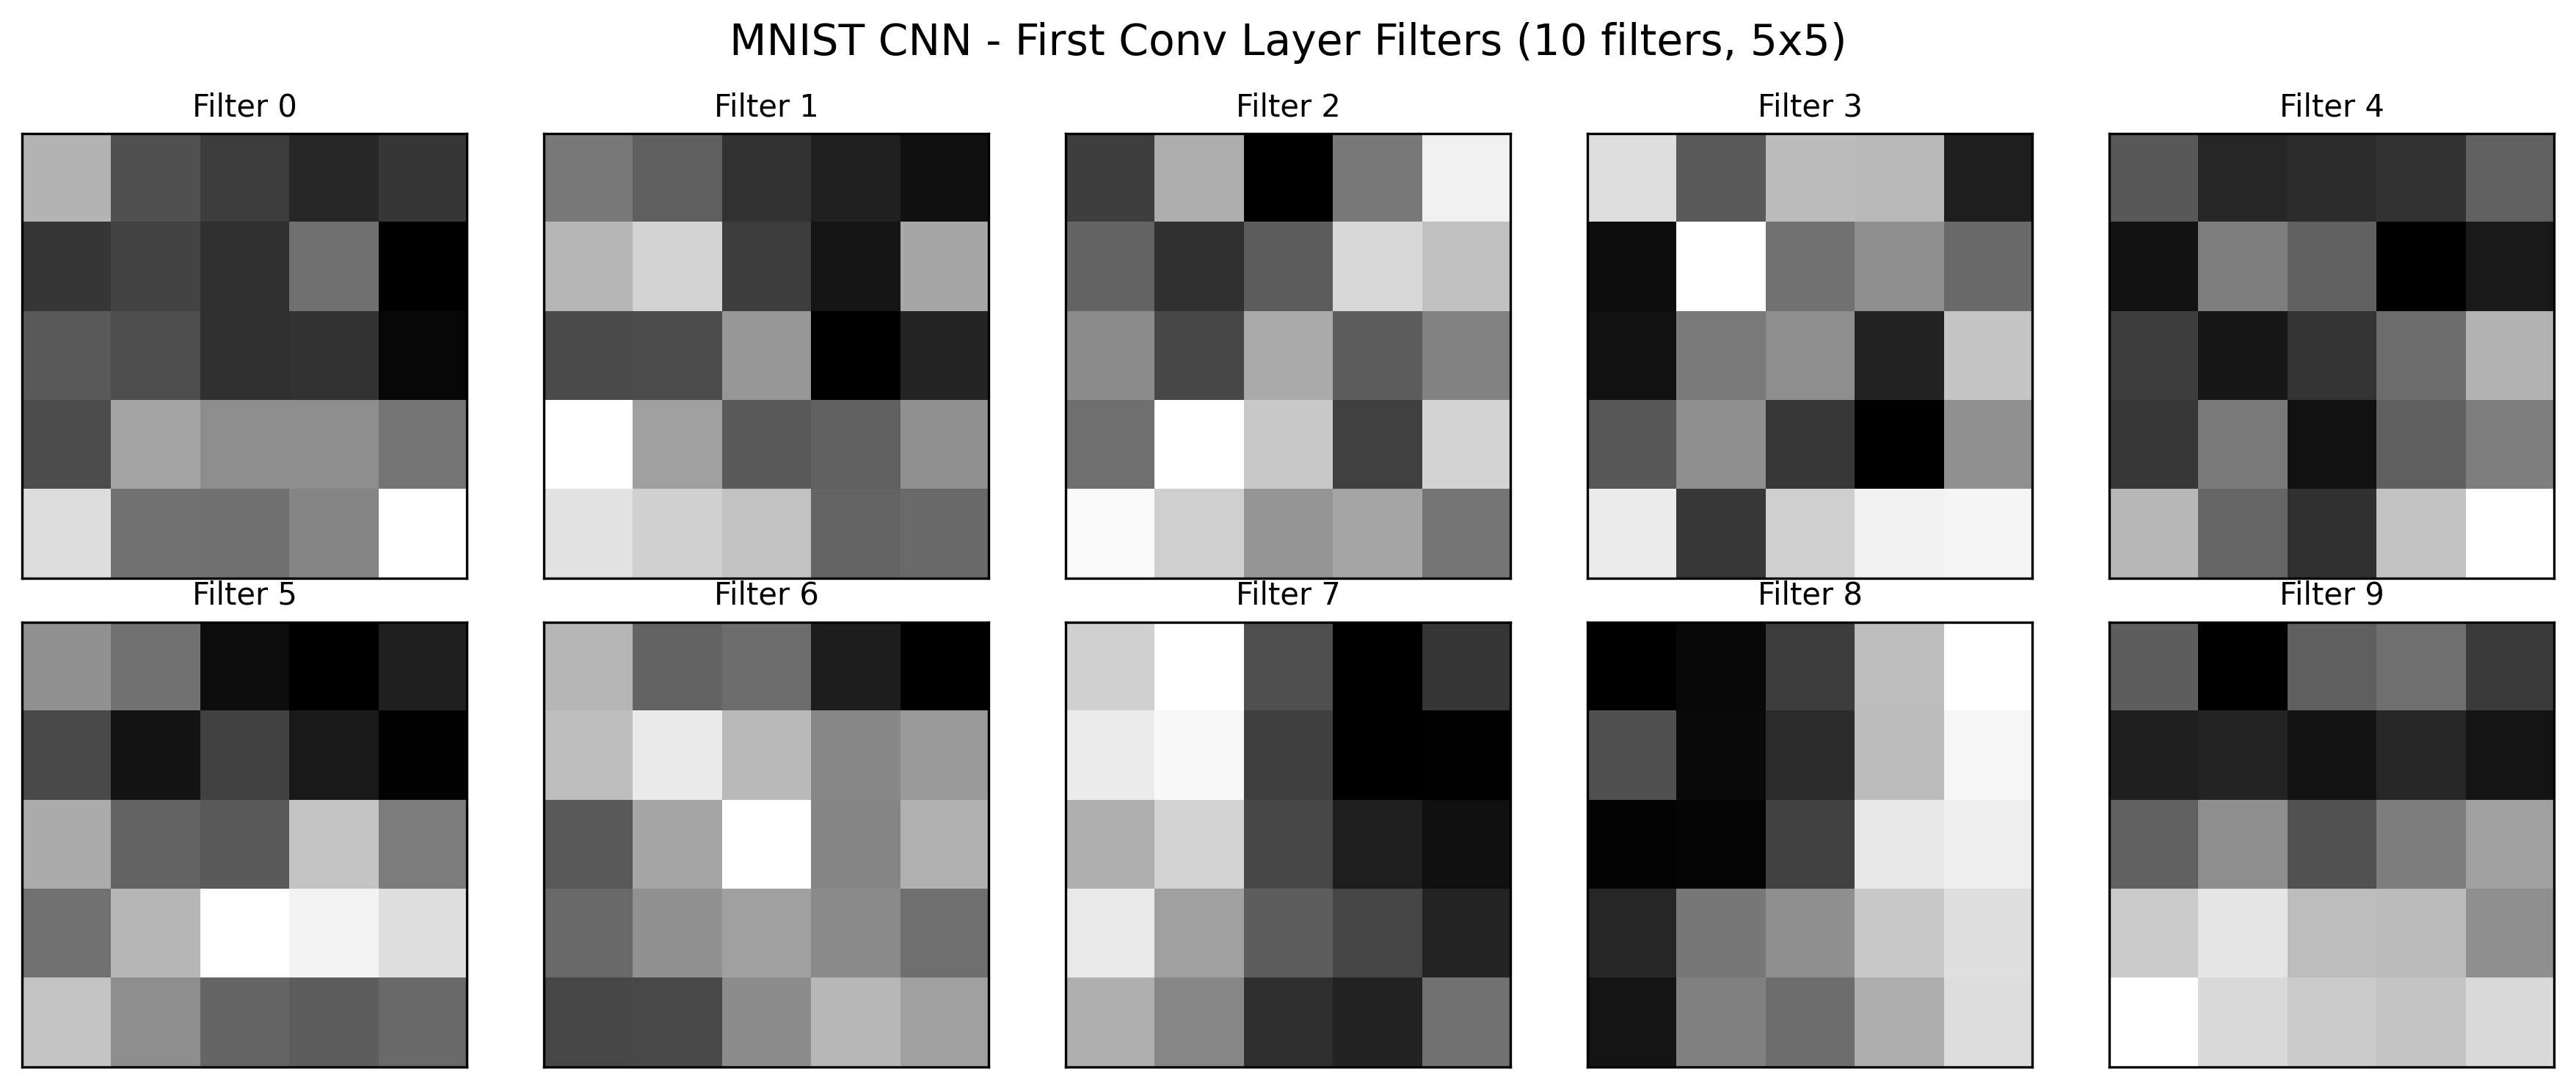
\includegraphics[width=0.75\textwidth]{results/mnist_conv1_filters.png}
    \caption{All 10 filters from our MNIST CNN's first convolutional layer (5$\times$5, single channel). These filters capture basic stroke patterns relevant to digit recognition.}
\end{figure}

\begin{table}[H]
    \centering
    \caption{First Layer Filter Comparison: MNIST CNN vs.\ ResNet18}
    \vspace{0.1in}
    \begin{tabular}{lcc}
        \toprule
        \textbf{Metric} & \textbf{MNIST CNN} & \textbf{ResNet18} \\
        \midrule
        Number of filters & 10 & 64 \\
        Input channels & 1 (grayscale) & 3 (RGB) \\
        Filter size & 5$\times$5 & 7$\times$7 \\
        Total parameters & 250 & 9,408 \\
        Weight range & [-0.48, 0.48] & [-0.84, 1.02] \\
        Weight std & 0.204 & 0.130 \\
        \bottomrule
    \end{tabular}
\end{table}

\subsubsection{Analysis}

\begin{itemize}
    \item \textbf{ResNet18 filters} show clear, interpretable patterns: horizontal and vertical edge detectors, diagonal gradient filters, and center-surround (blob) detectors. These are general-purpose features learned from ImageNet's diverse natural images (1.2M images, 1000 classes).
    
    \item \textbf{MNIST CNN filters} are less structured because the task is simpler---recognizing white strokes on black backgrounds requires less feature diversity than natural image classification.
    
    \item \textbf{Weight distribution}: ResNet18 has a wider weight range but lower standard deviation (0.130 vs.\ 0.204), indicating more specialized, peaked filter responses. Our MNIST CNN's weights are more uniformly distributed.
    
    \item \textbf{Scale difference}: ResNet18 uses $\sim$38$\times$ more parameters in its first layer alone. This is necessary to capture the much greater visual complexity of natural images compared to handwritten digits.
\end{itemize}

\subsection{Extension B: Live Video Digit Recognition}

\subsubsection{Approach}

We built a real-time digit recognition application (\texttt{extension\_live\_video.py}) that deploys our trained MNIST CNN for live inference on a webcam feed. The goal was to explore the challenges of taking a model trained on curated data (MNIST) and deploying it on raw, real-world input.

\textbf{System Design:}
\begin{enumerate}
    \item \textbf{Camera Auto-Detection}: The application scans video device indices 0--4 to automatically find an available webcam, ensuring compatibility across different systems.
    
    \item \textbf{ROI-based Capture}: A bounding box in the center of the frame defines the region of interest (200$\times$200 pixels) where the user positions a digit.
    
    \item \textbf{Preprocessing Pipeline}: The ROI undergoes the same transformation used by the training pipeline:
    \begin{itemize}
        \item Grayscale conversion
        \item Gaussian blur (5$\times$5 kernel) to reduce noise
        \item Otsu's adaptive thresholding (auto-inverts to white-on-black)
        \item Resize to 28$\times$28 with area interpolation
        \item Normalization (mean=0.5, std=0.5)
    \end{itemize}
    
    \item \textbf{Real-time Inference}: Each frame is passed through the CNN, producing a prediction displayed in a color-coded bounding box---green ($>$70\% confidence), yellow (40--70\%), or red ($<$40\%).
    
    \item \textbf{Visual Overlays}: A probability bar chart for all 10 classes and a debug view of the preprocessed 28$\times$28 input are rendered on each frame.
\end{enumerate}

\subsubsection{Live Webcam Results}

We tested the application by holding up digit images on a phone screen in front of the webcam. The bounding box, prediction label, confidence percentage, and probability distribution are all rendered in real-time.

\begin{figure}[H]
    \centering
    \begin{minipage}{0.48\textwidth}
        \centering
        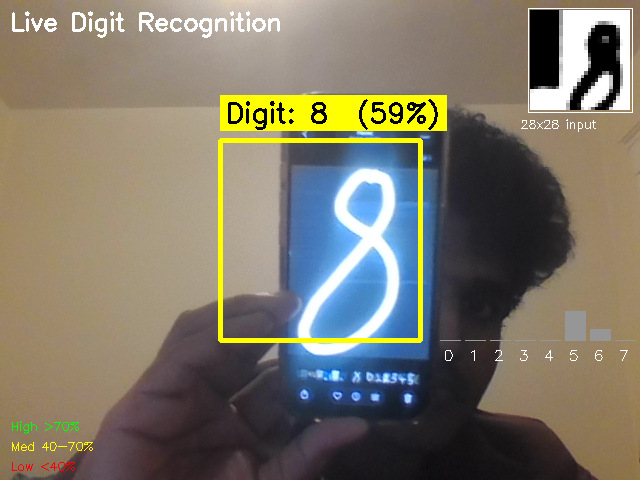
\includegraphics[width=\textwidth]{results/live_video/live_digit_1.png}
    \end{minipage}
    \hfill
    \begin{minipage}{0.48\textwidth}
        \centering
        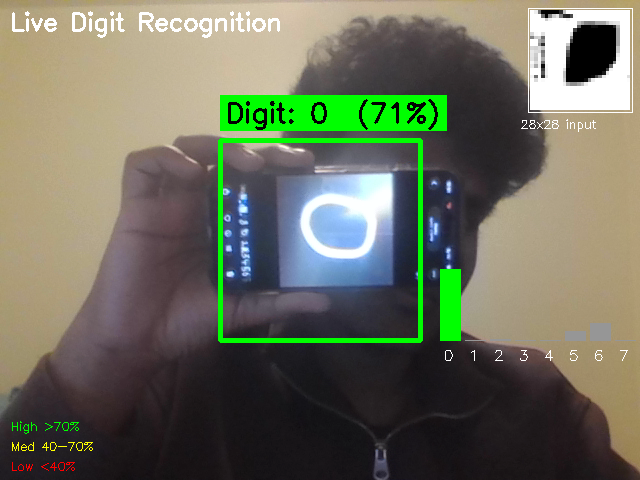
\includegraphics[width=\textwidth]{results/live_video/live_digit_3.png}
    \end{minipage}
    \caption{Live webcam digit recognition screenshots. The color-coded bounding box (green = high confidence, yellow = medium, red = low) surrounds the ROI. The predicted digit and confidence are shown above the box, with a class probability bar chart on the right and the preprocessed 28$\times$28 input in the top-right corner.}
\end{figure}

\begin{figure}[H]
    \centering
    \begin{minipage}{0.48\textwidth}
        \centering
        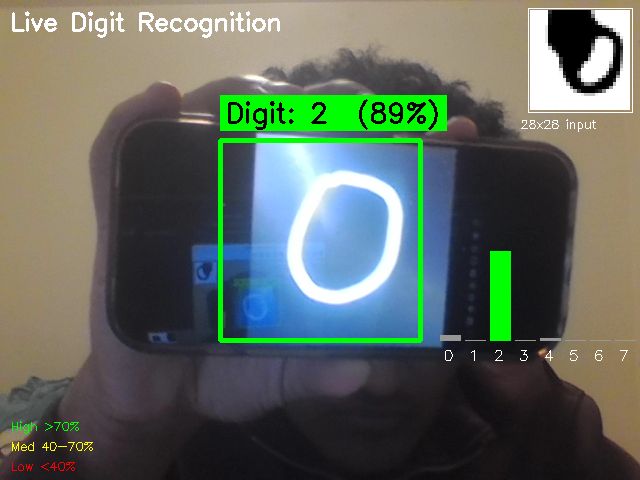
\includegraphics[width=\textwidth]{results/live_video/live_digit_5.png}
    \end{minipage}
    \hfill
    \begin{minipage}{0.48\textwidth}
        \centering
        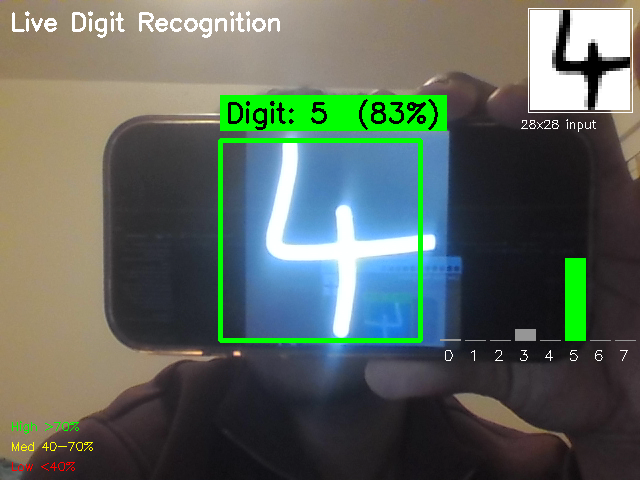
\includegraphics[width=\textwidth]{results/live_video/live_digit_7.png}
    \end{minipage}
    \caption{Additional live recognition results. The debug view (top-right corner of each frame) shows exactly what the network sees after preprocessing, allowing us to verify that the Otsu thresholding correctly isolates the digit.}
\end{figure}

\subsubsection{Analysis}

The live demo revealed several practical insights about deploying neural networks in the real world:

\begin{itemize}
    \item \textbf{Confidence-based feedback}: The color-coded bounding box gives immediate visual feedback on prediction reliability. Many predictions fall in the yellow/red range, reflecting the domain gap between MNIST and webcam input.
    
    \item \textbf{Preprocessing is critical}: The debug view revealed that Otsu's thresholding sometimes captures background artifacts (screen glare, hand edges), corrupting the 28$\times$28 input the network receives. Better preprocessing (e.g., contour-based cropping, morphological operations) could improve accuracy.
    
    \item \textbf{Domain gap}: Even when digits are clearly visible to human eyes, the network may be uncertain because MNIST digits have specific stroke characteristics (thin, centered, uniform) that differ from phone-displayed or hand-drawn digits in a webcam setting.
    
    \item \textbf{Real-time feasibility}: Inference runs at full webcam framerate ($\sim$30 fps) since the CNN is small (21,840 parameters), demonstrating that even simple models can be deployed for real-time applications.
\end{itemize}

\section{Reflection}

This project provided hands-on experience with two fundamentally different deep learning architectures for image classification. Building the CNN taught us how convolution layers extract hierarchical features—edges in early layers, shapes in deeper layers—and how components like max pooling, dropout, and batch processing work together during training.

Re-implementing the task with a Vision Transformer revealed how attention mechanisms can replace convolutions entirely. The process of splitting images into patches, creating token embeddings, and using self-attention to capture global relationships offered a different perspective on feature extraction. Comparing the two architectures deepened our understanding of inductive biases—CNNs assume local spatial correlations, while transformers learn all relationships from data.

Testing on custom handwritten digits highlighted the importance of data distribution matching. The domain gap between MNIST's training data and our handwriting style caused several misclassifications, demonstrating that neural networks are only as good as their training data and that real-world deployment requires careful attention to data preprocessing and augmentation.

\section{Acknowledgements}

\begin{itemize}
    \item \textbf{PyTorch and torchvision}: Used for model building, training, data loading, and preprocessing.
    \item \textbf{Professor's Notes}: Course materials and the NetTransformer template provided guidance on network architecture and transformer implementation.
    \item \textbf{PyTorch Tutorials}: Referenced for training loop structure and best practices.
    \item \textbf{Google Gemini}: Used as a research and debugging tool for understanding PyTorch functions and transformer architecture details.
\end{itemize}

\end{document}
